\PassOptionsToPackage{unicode=true}{hyperref} % options for packages loaded elsewhere
\PassOptionsToPackage{hyphens}{url}
\PassOptionsToPackage{dvipsnames,svgnames*,x11names*}{xcolor}
%
\documentclass[paper=a4,justified,a4paper]{tufte-handout}
\usepackage{lmodern}
\usepackage{amssymb,amsmath}
\usepackage{ifxetex,ifluatex}
\usepackage{fixltx2e} % provides \textsubscript
\ifnum 0\ifxetex 1\fi\ifluatex 1\fi=0 % if pdftex
  \usepackage[T1]{fontenc}
  \usepackage[utf8]{inputenc}
  \usepackage{textcomp} % provides euro and other symbols
\else % if luatex or xelatex
  \usepackage{unicode-math}
  \defaultfontfeatures{Ligatures=TeX,Scale=MatchLowercase}
\fi
% use upquote if available, for straight quotes in verbatim environments
\IfFileExists{upquote.sty}{\usepackage{upquote}}{}
% use microtype if available
\IfFileExists{microtype.sty}{%
\usepackage[]{microtype}
\UseMicrotypeSet[protrusion]{basicmath} % disable protrusion for tt fonts
}{}
\IfFileExists{parskip.sty}{%
\usepackage{parskip}
}{% else
\setlength{\parindent}{0pt}
\setlength{\parskip}{6pt plus 2pt minus 1pt}
}
\usepackage{xcolor}
\usepackage{hyperref}
\hypersetup{
            pdftitle={Evaluate your coaching skills - Reflection Report},
            pdfauthor={Helena Rasche},
            colorlinks=true,
            linkcolor=Maroon,
            filecolor=Maroon,
            citecolor=Blue,
            urlcolor=Blue,
            breaklinks=true}
\urlstyle{same}  % don't use monospace font for urls
\usepackage{longtable,booktabs}
% Fix footnotes in tables (requires footnote package)
\IfFileExists{footnote.sty}{\usepackage{footnote}\makesavenoteenv{longtable}}{}
\usepackage{graphicx,grffile}
\makeatletter
\def\maxwidth{\ifdim\Gin@nat@width>\linewidth\linewidth\else\Gin@nat@width\fi}
\def\maxheight{\ifdim\Gin@nat@height>\textheight\textheight\else\Gin@nat@height\fi}
\makeatother
% Scale images if necessary, so that they will not overflow the page
% margins by default, and it is still possible to overwrite the defaults
% using explicit options in \includegraphics[width, height, ...]{}
\setkeys{Gin}{width=\maxwidth,height=\maxheight,keepaspectratio}
\setlength{\emergencystretch}{3em}  % prevent overfull lines
\providecommand{\tightlist}{%
  \setlength{\itemsep}{0pt}\setlength{\parskip}{0pt}}
\setcounter{secnumdepth}{0}
% Redefines (sub)paragraphs to behave more like sections
\ifx\paragraph\undefined\else
\let\oldparagraph\paragraph
\renewcommand{\paragraph}[1]{\oldparagraph{#1}\mbox{}}
\fi
\ifx\subparagraph\undefined\else
\let\oldsubparagraph\subparagraph
\renewcommand{\subparagraph}[1]{\oldsubparagraph{#1}\mbox{}}
\fi

% set default figure placement to htbp
\makeatletter
\def\fps@figure{htbp}
\makeatother

\usepackage{pdfpages}

%%%%%%%%%%% Header and Footer %%%%%%%%%%%%%%%%%%
\fancyfoot[CE,CO]{\flushright 
\includegraphics[width=3cm]{../avans.jpg}}
\fancyhead[CE,CO]{\flushleft \smallcaps{\today}}


\title{Evaluate your coaching skills - Reflection Report}
\author{Helena Rasche}
\date{2022-02-07}

\begin{document}
\maketitle
\begin{abstract}
As the pandemic continues and lessons continue online, my primary
concern is that students are getting the support they need and feeling
supported. Following the experiences during BDB and with finally
beginning the period(s) during which I teach students, I've discovered a
number of points which I should remind myself of regularly as
preparation for each lesson.
\end{abstract}
\noindent\rule{5in}{0.4pt}


\hypertarget{points-of-attention}{%
\section{Points of Attention}\label{points-of-attention}}

Given that my lessons continue to be online, I find myself quite
concerned about whether or not students are getting enough support and
personal attention, and receiving it in ways that work optimally for
them. I know that students can feel significantly isolated with working
from home constantly, and that I want to ensure that I'm a friendly and
accepting person that they feel comfortable contacting when they have
issues. Specifically I've heard occasionally that I go too quickly and
sought their suggestions for how to fix this--I don't notice it unless
someone says it, and I'd rather they say it at the time it's happening.

\hypertarget{questionnaire}{%
\section{Questionnaire}\label{questionnaire}}

I designed the enquête to measure a couple aspects of this
communication:

\begin{itemize}
\tightlist
\item
  Preferred method(s)
\item
  Preferred interaction modalities
\item
  Their experiences as students in my class
\item
  And their feelings on my interactions with them until now.
\end{itemize}

These aspects I found to be particularly important to me and my
interactions with students. I elaborated these with the following survey
design:

\begin{longtable}[]{@{}lll@{}}
\toprule
\begin{minipage}[b]{0.09\columnwidth}\raggedright
Question\strut
\end{minipage} & \begin{minipage}[b]{0.14\columnwidth}\raggedright
Aspect\strut
\end{minipage} & \begin{minipage}[b]{0.68\columnwidth}\raggedright
Text\strut
\end{minipage}\tabularnewline
\midrule
\endhead
\begin{minipage}[t]{0.09\columnwidth}\raggedright
1\strut
\end{minipage} & \begin{minipage}[t]{0.14\columnwidth}\raggedright
Question\strut
\end{minipage} & \begin{minipage}[t]{0.68\columnwidth}\raggedright
How comfortable do you feel discussing course questions, issues,
programming questions via\strut
\end{minipage}\tabularnewline
\begin{minipage}[t]{0.09\columnwidth}\raggedright
1\strut
\end{minipage} & \begin{minipage}[t]{0.14\columnwidth}\raggedright
Description\strut
\end{minipage} & \begin{minipage}[t]{0.68\columnwidth}\raggedright
Example questions include: where's the course recording, why is my code
failing, what do you mean I need to import that first\strut
\end{minipage}\tabularnewline
\begin{minipage}[t]{0.09\columnwidth}\raggedright
1\strut
\end{minipage} & \begin{minipage}[t]{0.14\columnwidth}\raggedright
Answer\strut
\end{minipage} & \begin{minipage}[t]{0.68\columnwidth}\raggedright
A choice matrix of {[}Email, Teams Text Chat, Teams Video Chat, In
person{]} and {[}Please no!, If I must, Meh, It's ok, Yes please, My
preferred way!{]}\strut
\end{minipage}\tabularnewline
\begin{minipage}[t]{0.09\columnwidth}\raggedright
2\strut
\end{minipage} & \begin{minipage}[t]{0.14\columnwidth}\raggedright
Question\strut
\end{minipage} & \begin{minipage}[t]{0.68\columnwidth}\raggedright
I find online classes \ldots{}.\strut
\end{minipage}\tabularnewline
\begin{minipage}[t]{0.09\columnwidth}\raggedright
2\strut
\end{minipage} & \begin{minipage}[t]{0.14\columnwidth}\raggedright
Description\strut
\end{minipage} & \begin{minipage}[t]{0.68\columnwidth}\raggedright
1 = They work great for me! 5 = It's so exhausted I hate it here\strut
\end{minipage}\tabularnewline
\begin{minipage}[t]{0.09\columnwidth}\raggedright
2\strut
\end{minipage} & \begin{minipage}[t]{0.14\columnwidth}\raggedright
Answer\strut
\end{minipage} & \begin{minipage}[t]{0.68\columnwidth}\raggedright
Likert-type scale (1-5)\strut
\end{minipage}\tabularnewline
\begin{minipage}[t]{0.09\columnwidth}\raggedright
3\strut
\end{minipage} & \begin{minipage}[t]{0.14\columnwidth}\raggedright
Question\strut
\end{minipage} & \begin{minipage}[t]{0.68\columnwidth}\raggedright
How do you feel about\strut
\end{minipage}\tabularnewline
\begin{minipage}[t]{0.09\columnwidth}\raggedright
3\strut
\end{minipage} & \begin{minipage}[t]{0.14\columnwidth}\raggedright
Answer\strut
\end{minipage} & \begin{minipage}[t]{0.68\columnwidth}\raggedright
Choice matrix of {[}Breakout rooms, being randomly called on, being
predictably called on, Kahoots / Competitive quizzes{]} and feeling
matrix of {[}Hate it, Meh, It's fun{]}\strut
\end{minipage}\tabularnewline
\begin{minipage}[t]{0.09\columnwidth}\raggedright
4\strut
\end{minipage} & \begin{minipage}[t]{0.14\columnwidth}\raggedright
Question\strut
\end{minipage} & \begin{minipage}[t]{0.68\columnwidth}\raggedright
Helena wants to discuss my solution in front of the class, that makes me
feel\strut
\end{minipage}\tabularnewline
\begin{minipage}[t]{0.09\columnwidth}\raggedright
4\strut
\end{minipage} & \begin{minipage}[t]{0.14\columnwidth}\raggedright
Answer\strut
\end{minipage} & \begin{minipage}[t]{0.68\columnwidth}\raggedright
Free text\strut
\end{minipage}\tabularnewline
\begin{minipage}[t]{0.09\columnwidth}\raggedright
5\strut
\end{minipage} & \begin{minipage}[t]{0.14\columnwidth}\raggedright
Question\strut
\end{minipage} & \begin{minipage}[t]{0.68\columnwidth}\raggedright
Some of you have commented I go too quickly, how can we address
this?\strut
\end{minipage}\tabularnewline
\begin{minipage}[t]{0.09\columnwidth}\raggedright
5\strut
\end{minipage} & \begin{minipage}[t]{0.14\columnwidth}\raggedright
Description\strut
\end{minipage} & \begin{minipage}[t]{0.68\columnwidth}\raggedright
I'm guessing you don't want to publicly speak up? Would you want to
message the TOA who can ask me to slow down? Is there something I can do
to make you feel ok asking me to slow down in front of your peers? (I
need the reminder, I get too focused on covering content, for
sure.)\strut
\end{minipage}\tabularnewline
\begin{minipage}[t]{0.09\columnwidth}\raggedright
5\strut
\end{minipage} & \begin{minipage}[t]{0.14\columnwidth}\raggedright
Answer\strut
\end{minipage} & \begin{minipage}[t]{0.68\columnwidth}\raggedright
Free text\strut
\end{minipage}\tabularnewline
\begin{minipage}[t]{0.09\columnwidth}\raggedright
6\strut
\end{minipage} & \begin{minipage}[t]{0.14\columnwidth}\raggedright
Question\strut
\end{minipage} & \begin{minipage}[t]{0.68\columnwidth}\raggedright
I feel like part of the class when ?\strut
\end{minipage}\tabularnewline
\begin{minipage}[t]{0.09\columnwidth}\raggedright
6\strut
\end{minipage} & \begin{minipage}[t]{0.14\columnwidth}\raggedright
Description\strut
\end{minipage} & \begin{minipage}[t]{0.68\columnwidth}\raggedright
i.e.~specific types of activities (and that I'm getting something more
useful out of being here rather than doing chores or something
else.)\strut
\end{minipage}\tabularnewline
\begin{minipage}[t]{0.09\columnwidth}\raggedright
6\strut
\end{minipage} & \begin{minipage}[t]{0.14\columnwidth}\raggedright
Answer\strut
\end{minipage} & \begin{minipage}[t]{0.68\columnwidth}\raggedright
Free text\strut
\end{minipage}\tabularnewline
\begin{minipage}[t]{0.09\columnwidth}\raggedright
7\strut
\end{minipage} & \begin{minipage}[t]{0.14\columnwidth}\raggedright
Question\strut
\end{minipage} & \begin{minipage}[t]{0.68\columnwidth}\raggedright
Any other remarks?\strut
\end{minipage}\tabularnewline
\begin{minipage}[t]{0.09\columnwidth}\raggedright
7\strut
\end{minipage} & \begin{minipage}[t]{0.14\columnwidth}\raggedright
Answer\strut
\end{minipage} & \begin{minipage}[t]{0.68\columnwidth}\raggedright
Free text\strut
\end{minipage}\tabularnewline
\begin{minipage}[t]{0.09\columnwidth}\raggedright
8\strut
\end{minipage} & \begin{minipage}[t]{0.14\columnwidth}\raggedright
Question\strut
\end{minipage} & \begin{minipage}[t]{0.68\columnwidth}\raggedright
Are you getting the support you need? Do you have the resources you
need?\strut
\end{minipage}\tabularnewline
\begin{minipage}[t]{0.09\columnwidth}\raggedright
8\strut
\end{minipage} & \begin{minipage}[t]{0.14\columnwidth}\raggedright
Answer\strut
\end{minipage} & \begin{minipage}[t]{0.68\columnwidth}\raggedright
Likert-type scale with stars (1-5)\strut
\end{minipage}\tabularnewline
\begin{minipage}[t]{0.09\columnwidth}\raggedright
9\strut
\end{minipage} & \begin{minipage}[t]{0.14\columnwidth}\raggedright
Question\strut
\end{minipage} & \begin{minipage}[t]{0.68\columnwidth}\raggedright
Final Remarks?\strut
\end{minipage}\tabularnewline
\begin{minipage}[t]{0.09\columnwidth}\raggedright
9\strut
\end{minipage} & \begin{minipage}[t]{0.14\columnwidth}\raggedright
Answer\strut
\end{minipage} & \begin{minipage}[t]{0.68\columnwidth}\raggedright
Free text\strut
\end{minipage}\tabularnewline
\bottomrule
\end{longtable}

\hypertarget{results}{%
\section{Results}\label{results}}

\textbf{Question 1}: This focused on communication, which gave rather
optimistic responses for the second year of a pandemic, as seen in
Figure \ref{fig:q1}.

\begin{figure}
\centering
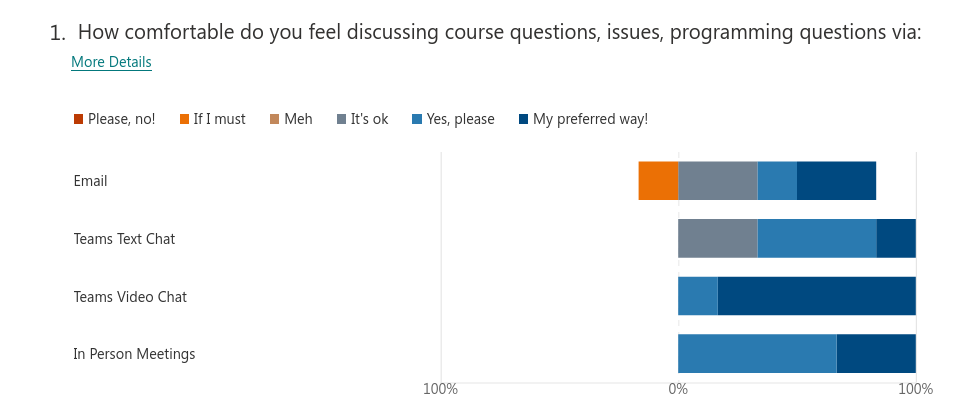
\includegraphics{q1.png}
\caption{Students seem to be extremely comfortable with online
communication, many just want to see a face clearly as video chat was
rated even more highly than in-person meetings which is expected for my
section of students as they were the half of the class which did not
require in-person learning in a start of period survey.\label{fig:q1}}
\end{figure}

\textbf{Question 2}: Students overall rated online classes as an ok
experience (min=1, mean=2, max=4, sd=1), only one student gave a higher
rating of 4 out of 5 (five being they're exhausted and hate it online),
but this shows suboptimal study design as I've conflated ``lack of
enjoyment'' and ``exhaustion'' which I expect many of us are
experiencing, and it's unclear \emph{why} the student responded like
they did.

\textbf{Question 3}: This question answers an important point for me,
that students are enjoying the new teaching methods implemented and
discussed in Assignment 10, breakout rooms where they do
pair-programming. Results in Figure \ref{fig:q3}.

\begin{figure}
\centering
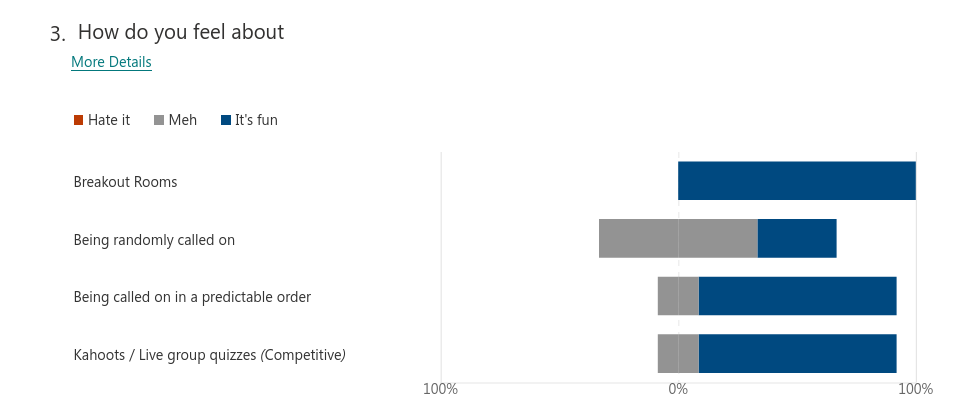
\includegraphics{./q3.png}
\caption{How do you feel about: a selection of activities and
methodologies\label{fig:q3}}
\end{figure}

\textbf{Question 4}: The variety of responses have been interesting to
say the least. To summarize the main points of the students:

\begin{itemize}
\tightlist
\item
  Some worried because they were beginners, and know that their answer
  won't be correct.
\item
  Some feel very seen, that the teacher takes time to interact and
  discuss their answer.
\item
  Most felt ok with it, knowing that it was a necessary part of the
  learning process.
\end{itemize}

Seeing these responses, and given that this is a technical course where
we have a significant amount of control over where the students execute
code, I've asked my TOA to look into automating the collection of
student solutions to a given problem in a way that I can use it
dynamically during class. That will allow me to discuss student
solutions with the class anonymously and maybe achieve everyone's
objectives: no hurt feelings, no uncomfortable attention, and the
student's solutions we review will still feel seen.

\textbf{Question 5}: This again gave food for thought on potential
options to slow down, some more actionable than others

\begin{itemize}
\tightlist
\item
  All steps should be repeated twice.
\item
  It's unclear when steps are something we need to run, or just for
  explanation.
\item
  I don't want to slow down just for me, knowing other people have the
  same issue helps
\item
  Sometimes you make a mistake, and catching up is tough, but the
  recording helps.
\item
  No problem with speed.
\end{itemize}

\textbf{Question 6}: Here I interrogated their community spirit, in case
there was anything I could do to help there

\begin{itemize}
\tightlist
\item
  Answering questions together (x3)
\item
  Breakout rooms \& Exercises (x3)
\item
  People speak up
\end{itemize}

I really appreciated the insight of one student's response there:

\begin{quote}
People need to be more interactive. Nobody responds when you ask a
question. {[}\ldots{}{]} But I think it also can be frustrating for you
that nobody is responding.
\end{quote}

Which I have to concur with.

\textbf{Question 7}: This had the most important point for me

\begin{itemize}
\tightlist
\item
  Lessons are great, sometimes a bit too fast
\item
  I really think you are a great teacher already to be honest!
\item
  I found it difficult to do the assignments with you 1:1, because I
  don't understand the assignments immediately and sometimes can feel
  like I am too slow.
\end{itemize}

That third point will be a focus of the reflection section below.

\textbf{Question 8}: Students were absolutely getting the support they
need (min=4, max=5, mean=4.666, stdev=0.47)

\textbf{Question 9}: The final other remarks section and not well
responded to, which is expected given that many people expressed
opinions in 6.

\hypertarget{reflection}{%
\section{Reflection}\label{reflection}}

\hypertarget{situation-review}{%
\subsection{Situation: Review}\label{situation-review}}

Numerous students across numerous questions, in this survey and the
previous, noted issues with the speed of lessons. Here either they
needed more review of individual things I mentioned (repeating
instructions) or more in depth discussion of the exercises which
students worked through on their own. While those exercises have
solutions available to students as they work through them, some
additional discussion is clearly beneficial.

\textbf{Looking Back}: During the times this happened during class I saw
no indication it was needed. No students reported it, the TOA didn't
mention it to me, and during exercises the students appeared to be
completing them at the expected pace and with the expected success rate.
I thought it was going ok for everyone, however their survey results
indicate they don't feel the same.

\textbf{Awareness}: To me this feels somewhere between an abject failure
(not knowing well enough what is going on with the students) and
perfectly acceptable (students won't get things immediately, and will
need to practice more later). This leaves me feeling a bit confused as
to what the real situation is. I value being approachable to students
which feels bad if they don't feel comfortable speaking up in front of
their peers when it's too fast.

\textbf{Alternatives}: In the future I can interrogate students more
regularly as to how they're feeling. This comes at the cost of precious
class time, but if the students answer and can give a more accurate
assessment of their feeling, then it's worth it. Additionally I can
embed more anonymous methods for feedback within the course days (either
via Teams or otherwise) to let students indicate their feelings of the
speed of the content and their understanding which comes at the expense
of more work, more setup time for classes required. However again, maybe
it produces a useful result which will make the extra time worth it.

\textbf{Trials}: I will start by going through the steps of every
exercise twice to help the students who feel like they got lost along
the way. Additionally I'll start regularly sending MS Forms polls in the
chat to ask how students are feeling and if it's an ok pace or too fast
or slow. I need to see if I can automate this, because it takes a bit of
time to setup which distracts from the class. I want to watch out that
it's actually an issue of me going too quickly, and not just students
keeping up but needing more review time than was available during class.

\hypertarget{situation-experience-gap}{%
\subsection{Situation: Experience Gap}\label{situation-experience-gap}}

During one class we had an odd number of students. I have been doing
breakout rooms exclusively with duos, as I wanted them to learn the
corporate skill of pair programming. Given the odd student count, I
decided I'd pair with the leftover student myself so they could be
included in the activity. I paired with two different students during
that class period, so, thankfully the student remains anonymous:

\begin{quote}
I found it difficult to do the assignments with you 1:1, because I don't
understand the assignments immediately and sometimes can feel like I am
too slow. It would have helped if I got a bit more time to try it myself
and read the question I think. (The 1:1 itself doesn't bother me tho)
\end{quote}

I should have paired them with someone on their own level, rather than
attempting to participate due the huge disparity in skill levels which
naturally led to blindspots where they did not understand the exercise
and I continued forward.

\textbf{Looking Back}: At the time I should have noticed. I attempted to
`play' an equal who wouldn't be confirming their understanding and would
expect them to ask about questions they had. This was a suboptimal
choice.

\textbf{Awareness}: This feels like a small failing as a teacher, I
should have known it would not work successfully and either put them in
a trio, or let them lead the entire experience rather than trying to
stay to pair programming. It was the obvious thing that would happen,
when pairing two people of vastly inequal skill levels, that one would
feel the desire to push forward no matter what. It goes against my core
values to give this student a poor learning experience and environment,
especially if they didn't feel comfortable enough to ask for more time
to understand the exercises.

\textbf{Alternatives}: In the future avoiding the situation in the first
place would be the most ideal option, to avoid any biases creeping into
the conversation or exchange. Given that it was a practice period, the
skill gap is insurmountable and impossible to address, so other options
must be sought. If trios (with more evidence) proves suboptimal, then I
can pair with students and allow them to lead the entire exercise, maybe
that will go more easily?

\textbf{Trials}: I will start by avoiding this situation where possible
while I collect more data on if trios are better or worse than duos. If
trios turn out to be worse, then I will start pairing them with the TOA
(for a smaller skill differential) and failing that with myself, but in
either of the latter two cases I will recommend the student drives the
exercise, and the TOA/teacher simply acts as facilitator.

\hypertarget{action-points}{%
\section{Action Points}\label{action-points}}

Based on the results obtained in this brief survey, I've formulated a
number of points of attention to focus on during the period:

\begin{itemize}
\tightlist
\item
  Go through questions at the end of each exercise section.
\item
  Go through student solutions anonymously and discuss common problems.
\item
  Do not pair with students, the knowledge gap is too significant,
  instead have them form trios.
\end{itemize}

These seem relatively easy things to control and focus on, which in my
opinion bodes well for the coming semester. If this is all that the
students disliked, then, it's probably going ok.

\end{document}
